% \documentclass[a4paper,11pt]{article}
% \usepackage[hyperref]{beamerarticle}

\documentclass[final]{beamer}

\usepackage[hangul]{kotex}
\usepackage{amsfonts,amsmath,xob-amssymb}

\usepackage{amsthm}
\newtheorem{defn}{Definition}
\newtheorem{thm}{Theorem}

\usepackage{cancel}
\graphicspath{{./_img/05/}}

\usepackage{graphicx}
\usepackage{media9}
\usepackage{tikz}
\usepackage{textpos}

\mode<presentation>{
	\usetheme{Madrid}
	\usecolortheme{default}
	\usefonttheme{professionalfonts}
}

\def\b{\boldsymbol}

\mode<article>{
\usepackage{fullpage}
}
\usepackage{ulem}

\newcommand{\bb}{\mathbb}
\newcommand{\bd}{\mathbf}
\newcommand{\p}{\partial}

\newcounter{saveenumi}
\newcommand{\seti}{\setcounter{saveenumi}{\value{enumi}}}
\newcommand{\conti}{\setcounter{enumi}{\value{saveenumi}}}

\newcommand{\mail}{\url{mailto:experiment.namun+2016f@gmail.com} }


\title{게임이론 Part 3}
\subtitle{게임의 기본 개념들 (게임이론, 진화, 그리고 협력)}
\author[조남운]{허준석$\rightarrow$이동한$\rightarrow$\emph{조남운}\\\mail}

\begin{document}
	
\begin{frame}[t]{}
	\titlepage
\end{frame}
%--- Next Frame ---%	

\begin{frame}[t]{목차}
	\tableofcontents
\end{frame}
%--- Next Frame ---%

\section{전개형 게임 2(Extensive Form Game 2)} % (fold)
\label{sec:extensive_game_2}

\begin{frame}[t]{정보집합 (Information Set)}
	\begin{columns}[c]
	\column{18em}
	\begin{itemize}
		\item 2번째 노드에서 $P2$가 어디 있는지 모를 때
		\item 이것은 무엇과 동일한 상황인가? 
		\item 이것을 NFG (Normal Form Game)으로 나타내본다면?
		\item 정보집합을 저렇게 그릴 수 있는 조건은? 
	\end{itemize}
	\column{12em}
	\hspace{-1em}
	\fbox{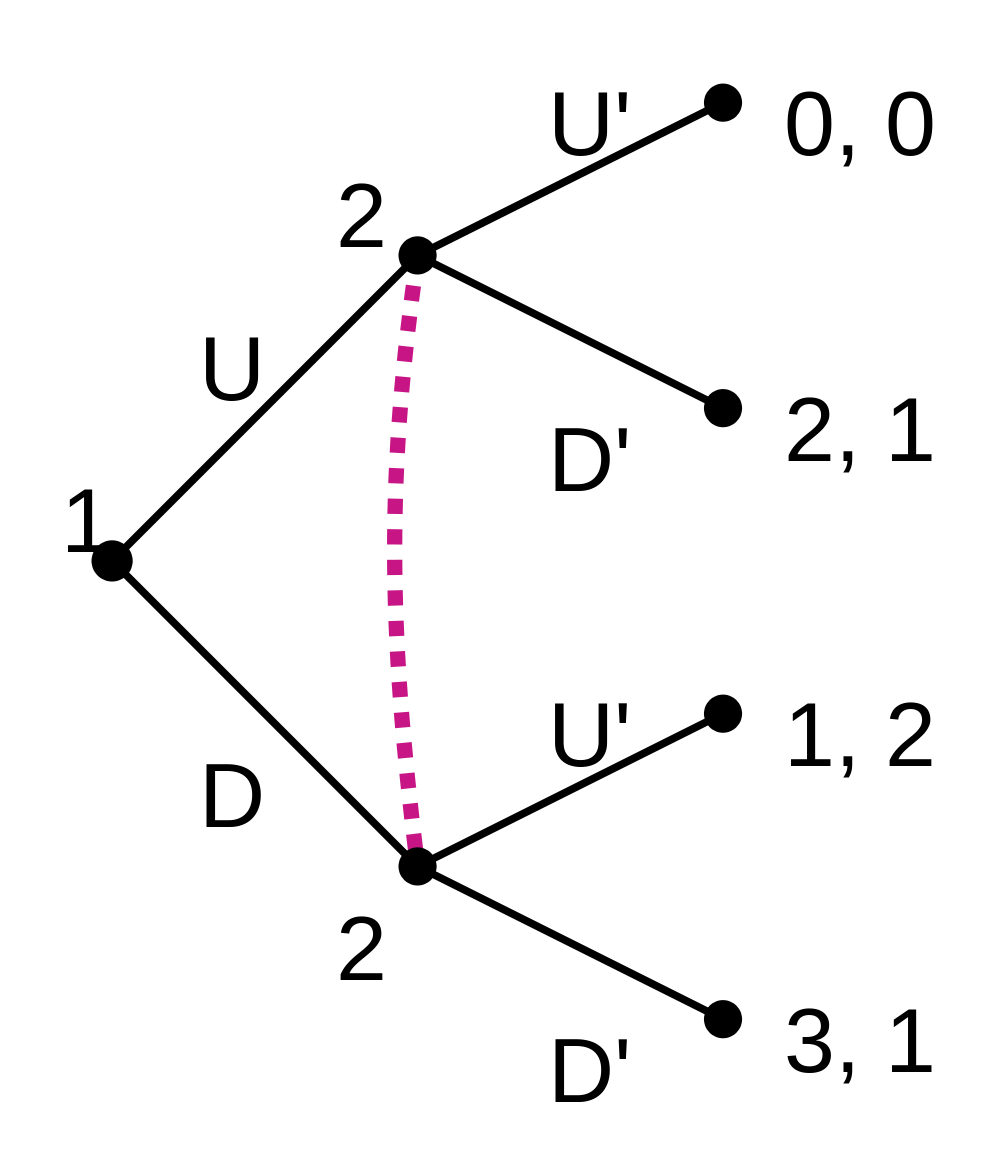
\includegraphics[width=11em]{efg_info.png}}
	\end{columns}
\end{frame}
%--- Next Frame ---%

\begin{frame}[t]{Exercise}
	\begin{columns}[c]
		\column{18em}
		\begin{itemize}
			\item Big John ($P1$) vs Little John ($P2$)
			\begin{enumerate}\small
				\item 옆의 NFG의 PSNE은 무엇인가? 
				\item 옆의 NFG의 MSNE은 무엇인가?
				\item Big John이 First mover일 때 EFG의 SPE (Subgame Perfect Equilibrium)은?
				\item Little John이 First mover일 때 EFG의 SPE은?
			\end{enumerate}
		\end{itemize}
		\column{12em}
		\begin{center}
			\begin{table}
				\setlength{\tabcolsep}{1.2em}
				\begin{tabular}{|c|c|c|} \hline
				& {C} &  {W} \\ \hline
				{C} & {$5$}, {$3$} & {$4$}, {$4$} \\ \hline%
				{W} & {$9$}, {$1$}  & {$0$}, {$0$} \\ 
				\hline
				\end{tabular}
			\end{table}
		\end{center}
	\end{columns}
\end{frame}
%--- Next Frame ---%

% section extensive_game_2 (end)

\section{Repeated Game (RG)} % (fold)
\label{sec:repeated_game}

\begin{frame}[t]{특별한 종류의 전개형 게임}
	%\begin{columns}[c]
	%\column{18em}
	\begin{itemize}
		\item 매기는 NFG 
		\item 전기의 결과에 의존해 다음 기가 진행 
		\item 전략의 수는? 
	\end{itemize}
	%\column{12em}
	\begin{center}
	\fbox{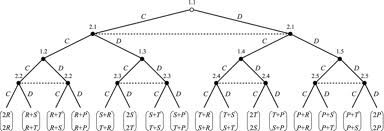
\includegraphics[width=27em]{rgame.jpeg}}
	\end{center}
	% \end{columns}
\end{frame}
%--- Next Frame ---%

\begin{frame}[t]{RG 실습}
	\begin{itemize}
		\item URL: 교실상에서 공지
	\end{itemize}
\end{frame}
%--- Next Frame ---%

\begin{frame}[t]{RG에서 균형은 어떻게 찾을까?}
	%\begin{columns}[c]
	%\column{13em}
	\begin{itemize}
		\item RG의 전략의 수는 너무 많다. 
		\item 기존의 방법으로는 찾기 힘들다. 
		\item 게다가, RG이 유한하게 전개된다면?
		\item BI (Backward Induction)에 따른 균형은 뻔한 결과 
	\end{itemize}
	%\column{16em}
	%\hspace{-1em}
	%\begin{center}
	%\fbox{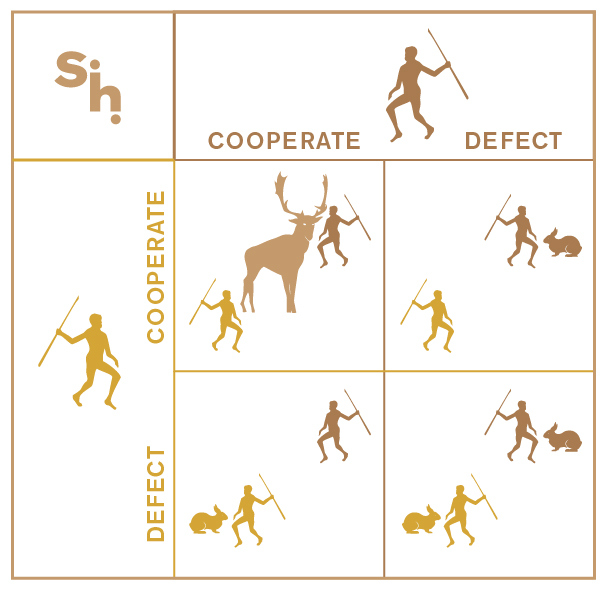
\includegraphics[width=13em]{staghunt.jpg}}
	%\end{columns}
\end{frame}
%--- Next Frame ---%

\begin{frame}\frametitle{Finite vs. Infinite}\vspace{3.5em}
%\begin{columns}[c]
%\column{13em}
\begin{itemize}
	\item Finitely repeated game에서 균형은 BI으로 
	\item Infinite repeated game에서 균형은? 
	\item 일단 전략이 다른 방식으로 주어져야 
\end{itemize}
%\column{16em}
%\hspace{-1em}
%\begin{center}
%\fbox{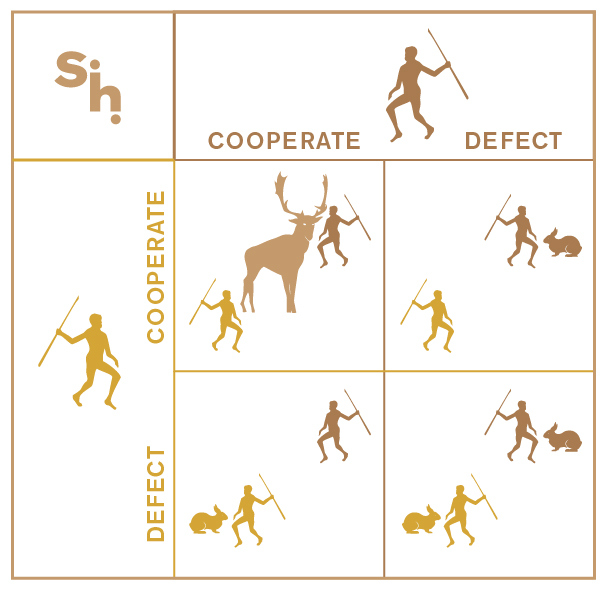
\includegraphics[width=13em]{staghunt.jpg}}
%\end{columns}
\end{frame}

\begin{frame}\frametitle{Chain-store Game in Finitely Repeated Game}\vspace{2em}
\begin{columns}[c]
\column{16em}
\begin{itemize}
	\item 20번에 걸쳐서 순차적으로 이 게임을 한다고 생각해보자. 즉, 1명의 현재 독점자와 20명의 순차적 경쟁자
	\item BI에 따른 균형은? 
	\item 하지만, chainstore는 협박을 통해 이윤을 늘릴 수 있다! 아마도 BI에 필요한 가정에 문제가 있는 것은 아닐까? 
\end{itemize}
\column{14em}\hspace{0em}
\fbox{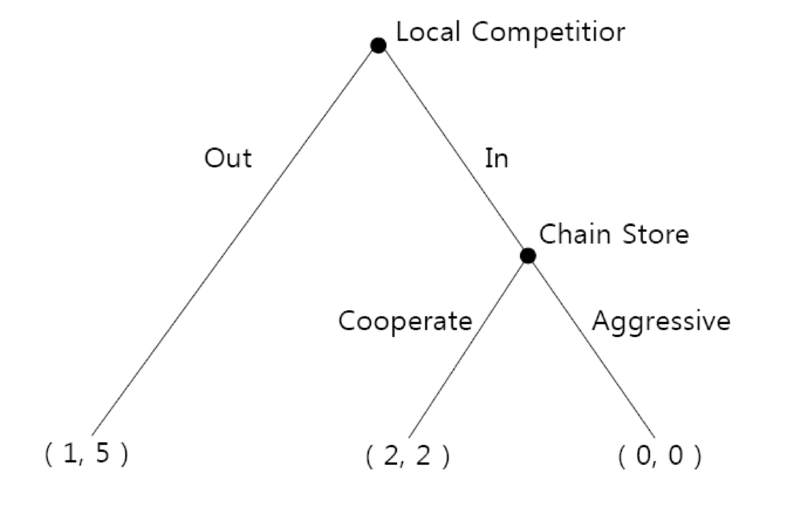
\includegraphics[width=14em]{chainstore01.png}}
\end{columns}
\end{frame}

\begin{frame}\frametitle{Strategy in Infinitely Repeated Games}\vspace{1em}
%\begin{columns}[c]
%\column{13em}
\begin{itemize}
	\item 전략은 algorithm 처럼 주어진다. 
	\item 즉, 상대의 전략에 의존적으로 주어진다. 
	\item 아울러 모든 결과를 정하기 힘들다면, 제한된 기억에 의존한다. 
	\item history matters. \\RG의 전략은 history에서 action으로 가는 함수
	\item RG의 전략들 
	\begin{enumerate}
		\item Tit-For-Tat (TFT)
		\item GRIM 
		\item Pablov (Win-Stay-Lose-Shift)
		\item ALLC / ALLD 
	\end{enumerate}
\end{itemize}
%\column{16em}
%\hspace{-1em}
%\begin{center}
%\fbox{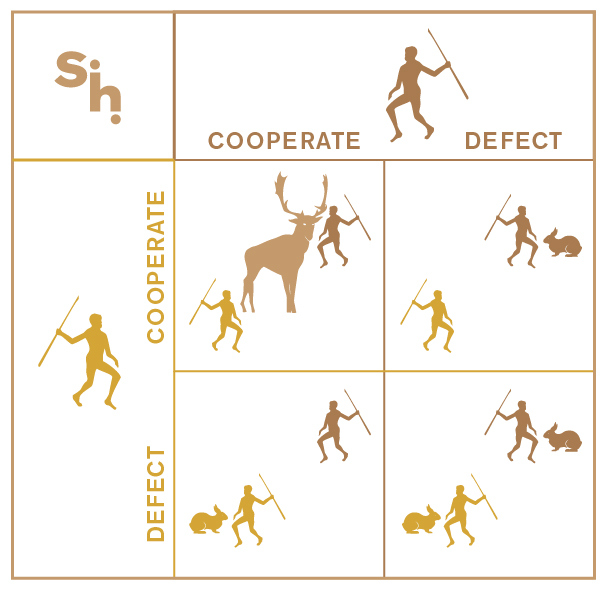
\includegraphics[width=13em]{staghunt.jpg}}
%\end{columns}
\end{frame}




\begin{frame}\frametitle{Payoff in Infinitely Repeated Games}\vspace{.5em}
%\begin{columns}[c]
%\column{13em}
\begin{itemize}
	\item 보수는 어떻게 정의되어야 할까? 
%
\begin{align*}
\overbrace{\Pi(s)}^{\ast}=\pi_1 (s) + \rho \times \pi_2 (s) + \rho^t \times \overbrace{\pi_t (s)}^{\ast\ast} + \ldots 
\end{align*}
%

	\begin{itemize}
		\item[$\ast$] 무한반복 게임의 보수 
		\item[$\ast\ast$] $t$기에 $s$ 전략에 따른 one-shot 보수 
	\end{itemize}

	\item $\rho$에 대한 해석: 

	\begin{enumerate}
		\item 시간 할인 (현재가치로 환산하기) 
		\item 같은 사람과 다음 기에 다시 만날 확률 
	\end{enumerate}

	\item $\Pi(s)$는 수렴해야 한다. 
	
\end{itemize}
%\column{16em}
%\hspace{-1em}
%\begin{center}
%\fbox{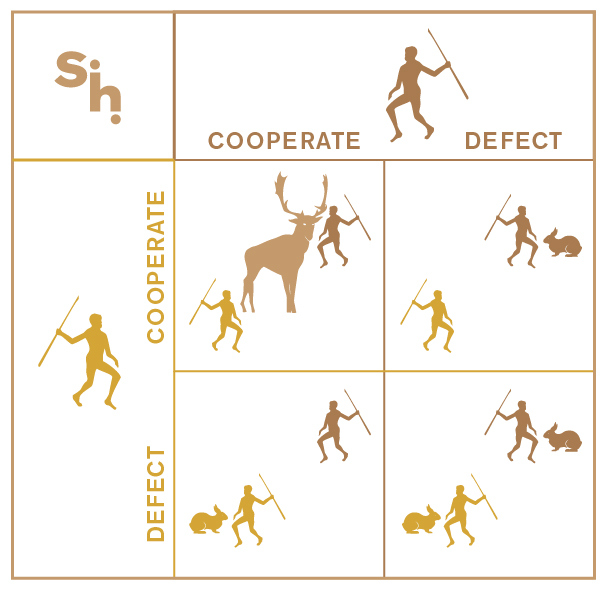
\includegraphics[width=13em]{staghunt.jpg}}
%\end{columns}
\end{frame}

\begin{frame}\frametitle{GRIM (Trigger) Strategy}\vspace{3.5em}
\begin{columns}[c]
\column{18em}
\begin{itemize}
	\item GRIM 전략은 다음과 같이 정의된다. 
	\item $\tau$ 기에 선수 $i$는 다음과 같이 전략을 선택한다. 
	\begin{enumerate}
		\item plays $C$ at $\tau=1$
		\item plays $C$, $\tau$ 이전 시기에 나와 남의 행동이 모두 $C$였다면
		\item plays $D$, 다른 모든 경우에 
	\end{enumerate}
	\item 왜 `Trigger' strategy인가? 
\end{itemize}
\column{13em}
\hspace{-1em}
\fbox{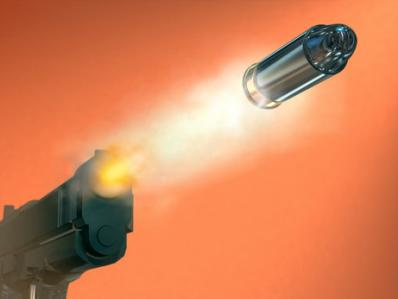
\includegraphics[width=13em]{gun.jpg}}
\end{columns}
\end{frame}

\begin{frame}\frametitle{TFT Strategy}\vspace{1em}
\begin{columns}[c]
\column{18em}
\begin{itemize}
	\item TFT 전략은 다음과 같이 정의된다. 
	\item $\tau$ 기에 선수 $i$는 다음과 같이 전략을 선택한다. 
	\begin{enumerate}
		\item plays $C$ at $\tau=1$
		\item 바로 전기에 상대의 행동을 plays 
	\end{enumerate}
	\item 로버트 액설로드, [협력의 진화] 
\end{itemize}
\column{13em}
\hspace{-1em}
\fbox{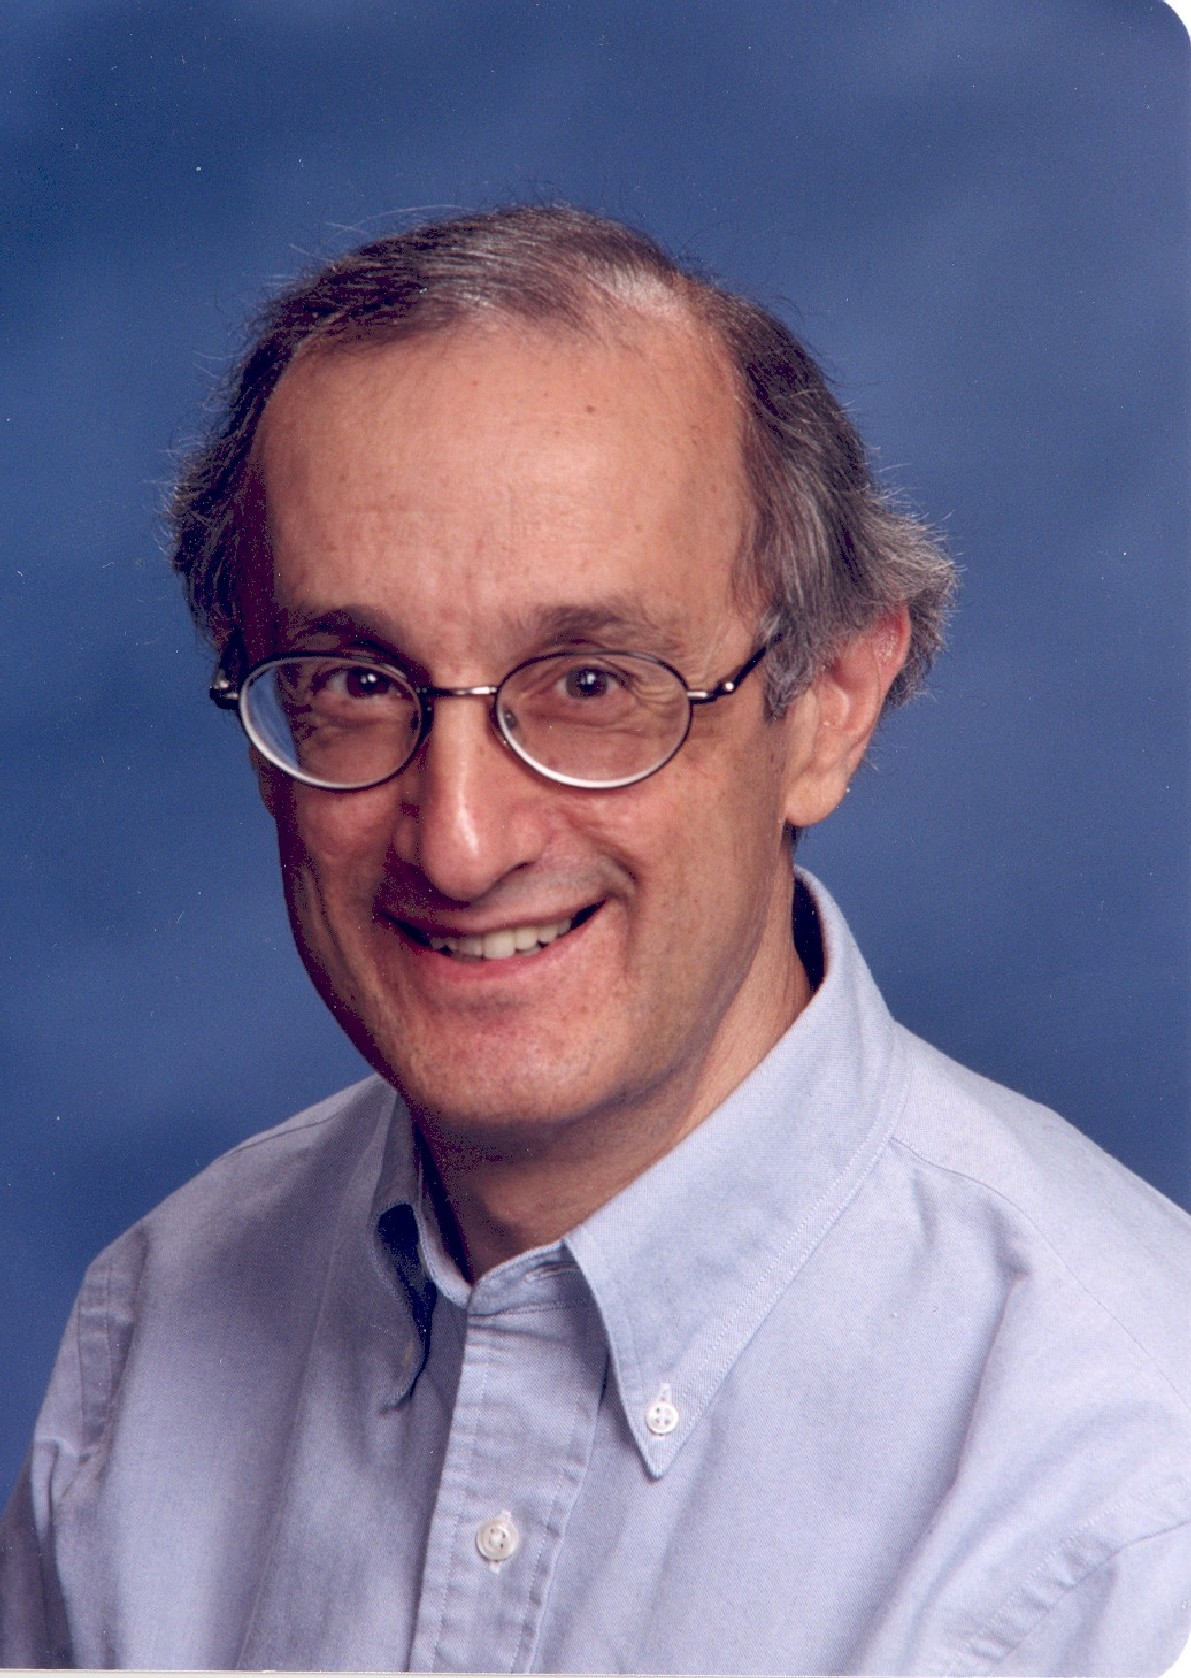
\includegraphics[width=13em]{raxelrod.jpg}}
\end{columns}
\end{frame}

\begin{frame}\frametitle{Back to PD Game!}\vspace{3.5em}
\begin{columns}[c]
\column{18em}
\begin{itemize}
	\item One-shot PDG 게임 혹은 finitely RPDG의 결론은? 
	\item 이러한 결론이 바뀌는 것이 가능할까?
	\item 만일 바뀐다면 어떤 것들이 영향을 주게 되는가? 
\end{itemize}
\column{13em}
\begin{table}
\setlength{\tabcolsep}{1.2em}
\begin{tabular}{|c|c|c|c|} \hline
& {C} &  {D}\\ \hline
{C} & {$2$}, {$2$} & {$0$}, {$3$} \\ \hline%
{D} & {$3$}, {$0$}  & {$1$}, {$1$}\\ 
\hline
\end{tabular}
\end{table}
\end{columns}
\end{frame}

\begin{frame}\frametitle{GRIM with IRPDG}\vspace{3.5em}
%\begin{columns}[c]
%\column{18em}
\begin{itemize}
\item  게임 상황 
	\begin{enumerate}
		\item GRIM에 입각한 두 명의 플레이어 
		\item 게임은 무한 반복
	\end{enumerate}
\item 만일 모두 GRIM을 따라서 움직인다면, 이때 선수들의 보수는?
%
\begin{align*}
\Pi = 2 + \rho \times 2 + \rho^2 \times 2 + \ldots 
\end{align*}
%
\end{itemize}
%\column{13em}
%\end{columns}
\end{frame}

\begin{frame}\frametitle{무한등비급수 계산하는 법}\vspace{1em}
%\begin{columns}[c]
%\column{18em}
\begin{itemize}
\item  초항이 $a$이고 공비가 $\rho$인 어떤 무한등비급수의 합이 $S$라고 하자. 즉,
%
\begin{align*}
S = a + \rho \times a + \rho^2 \times a + \cdots + \rho^t \times a \ldots 
\end{align*}
%
\item 이때 이 식은 다시 다음과 같이 정리될 수 있다. 
%
\begin{align*}
S = a + \rho \left( \overbrace{a + \rho^1 \times a + \ldots}^{=S} \right).
\end{align*}
%
\item 따라서, $S = \dfrac{a}{1-\rho}$. \\[0.8em]

\item 단, 저 값이 존재하려면 $\rho$는 어때야 할까? 
\end{itemize}
%\column{13em}
%\end{columns}
\end{frame}

\begin{frame}\frametitle{만일 플레이어가 GRIM을 따르지 않게 된다면?}\vspace{2em}
%\begin{columns}[c]
%\column{18em}
\begin{itemize}
\item  어떤 시점 $t$에서 선수가 GRIM을 따르지 않기로 했다고 쳐보자. 즉, 선수는 앞서 누구도 $D$를 하지 않았으나 $C$를 하는 대신 $D$를 했다고 해보자. 
%
\begin{align*}
\Pi' = \overbrace{2 + \rho \times 2 + \rho^{t-1} \times 2}^{\text{GRIM을 따를 때}} + \overbrace{\rho^t \times 3}^{\text{따르지않았을 때}} + \overbrace{\rho^{t+1} \times 1 + \ldots}^{\text{그 이후}}
\end{align*}
%
\item 만일 이러한 일탈이 발생하지 않으려면, 어떤 조건이 성립하면 될까? 
%
\begin{align*}
\Pi' > \Pi
\end{align*}
%
\end{itemize}
%\column{13em}
%\end{columns}
\end{frame}

\begin{frame}\frametitle{만일 플레이어가 GRIM을 따르지 않게 된다면?}\vspace{2em}
%\begin{columns}[c]
%\column{18em}
\begin{itemize}
\item 사실상 $t-1$까지는 모두가 GRIM에 충실했으므로 두 사람의 보수가 같을 것이다. 따라서, 이건 그냥 잘라내고 생각을 하자. 그리고 두 사람의 보수를 모두 $\rho^{t}$로 나누어보자. 
\item 결국 이는 어떤 플레이어가 게임이 시작되는 첫기에 GRIM에 따라서 움직이지 않았을 때의 보수와 이에 충실했을 때의 보수 사이의 비교의 문제가 된다. 
%
\item 결국 1회의 PDG과 다른 결과를 낳을 가능성을 부여하는 것은 무엇인가? 
\end{itemize}
%\column{13em}
%\end{columns}
\end{frame}

\begin{frame}\frametitle{한가지 이론적인 질문 (Optional)}\vspace{2em}
%\begin{columns}[c]
%\column{18em}
\begin{itemize}
\item 앞서서 반복게임이란 `특수한' 형태의 전개형 게임이라고 언급. 
\item 그런데, 전개형 게임에서 NE을 걸러내는 틀 중에서 유용하게 사용한 것은 무엇인가? 
\item 어떤 균형이 SPE가 되려면, 우리가 지나가지 않은 경로에서도 모두 최적으로 행동을 해야 한다. 즉, 만일 지나가지 않은 경로에서 그렇지 않게 행동했을 것이라면 BI에 따라서 원래 플레이어의 결정도 지금과 같지 않을 것이기 때문. 
\item 이 문제를 앞서에 응용해보자. 플레이어가 $C$를 하지 않고 $D$를 했을 경우에도 GRIM의 지시에 따르는 것이 플레이어에게 가장 좋은가? 
\end{itemize}
%\column{13em}
%\end{columns}
\end{frame}

\begin{frame}\frametitle{Conscientious GRIM?}\vspace{3em}
%\begin{columns}[c]
%\column{18em}
\begin{itemize}
\item 앞서 정의한 GRIM을 다음처럼 다시 정의해보자. 
\begin{enumerate}
		\item plays $C$ at $\tau=1$
		\item plays $C$, $\tau$ 이전 시기에 남의 행동이 모두 $C$였다면
		\item plays $D$, 다른 모든 경우에 
	\end{enumerate}
\item 이렇게 정의된 전략은 SPE인가? 
\end{itemize}
%\column{13em}
%\end{columns}
\end{frame}

\begin{frame}\frametitle{게임은 반복되어야 한다}\vspace{5mm}
\begin{itemize}\large
\item 정해진 횟수의 게임 : 역추론의 문제 발생\\
$\rightarrow$ 무임승차 전략
\item 고정된 확률로 게임이 반복 \\
$\rightarrow$ 다음회의 보복이 두려워 협조를 한다 \\
$\rightarrow$ 다음 회가 발생할 확률이 중요
\end{itemize}
\end{frame}

\begin{frame}\frametitle{상호성 가설에 의한 이타적 행위 모형 I}\vspace{5mm}
\begin{itemize}\large
%(1) 조건부 협조: 첫 회에 협조로 시작, 그 다음 회부터는 상대방이 전기에 협조를 한 경우에만 협조. 상대가 한 번이라도 배신하면 그 다음 부터 계속 배신 \\
\item 무조건 배신(ALLD): 첫 회부터 배신하는 것으로 시작해서 계속 배신 \\
\item 무조건 협조(ALLC): 첫 회부터 협조하는 것으로 시작해서 계속 배신
\end{itemize}
\begin{center}
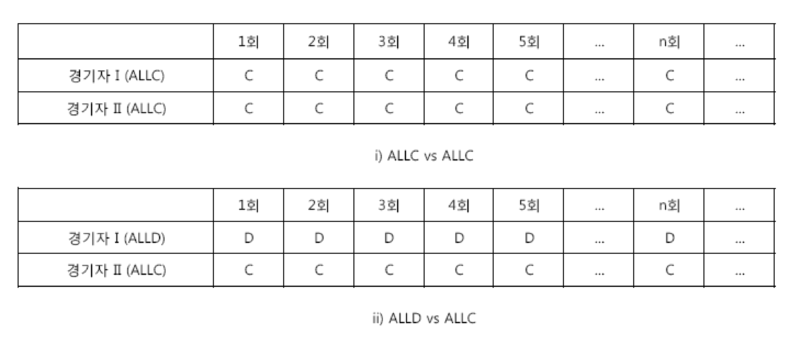
\includegraphics[width=4in]{alldallc01.png}
\end{center}
\end{frame}

\begin{frame}\frametitle{상호성 가설에 의한 이타적 행위 모형 II}%\vspace{5mm}
\begin{itemize}\large
\item 조건부 협조: 첫 회에 협조로 시작, 그 다음 회부터는 상대방이 전기에 협조를 한 경우에만 협조. 상대가 한 번이라도 배신하면 그 다음 부터 계속 배신 \\
%(2) 배신: 첫 회부터 배신을 하는 것으로 시작해서 계속 배신
\end{itemize}
\begin{center}
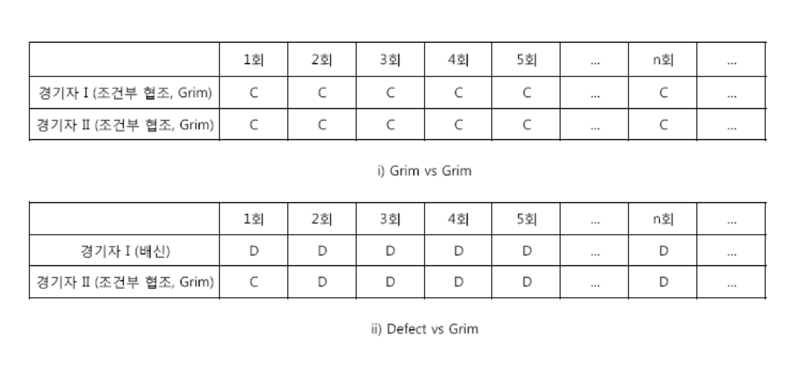
\includegraphics[width=4in]{condcoop01.png}
\end{center}
\end{frame}

\begin{frame}\frametitle{상호성 가설에 의한 이타적 행위 모형 III}\vspace{5mm}
\begin{itemize}\large
\item 게임이 반복될 확률이 $\delta$일 때 총보수
\end{itemize}
\begin{center}
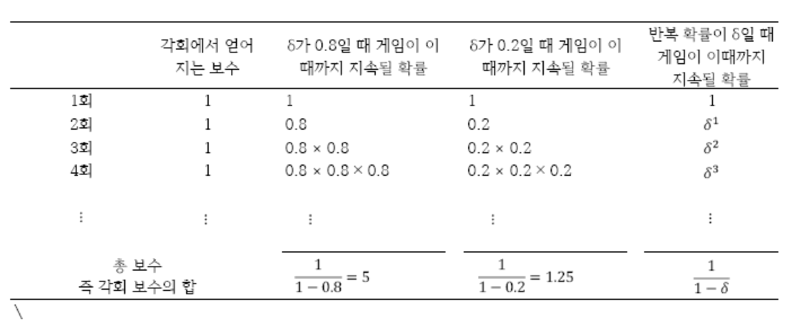
\includegraphics[width=4in]{repeatpayoff01.png}
\end{center}
\end{frame}

\begin{frame}\frametitle{상호성 가설에 의한 이타적 행위 모형 IV}%\vspace{5mm}
\begin{itemize}\large
\item $\dfrac{b-c}{1-\delta} > b \rightarrow \delta > \dfrac{c}{b} $ \\
조건부협조(Grim, Trigger)전략이 효과적이려면 높은 확률로 반복되어야 !!
\end{itemize}
\begin{center}
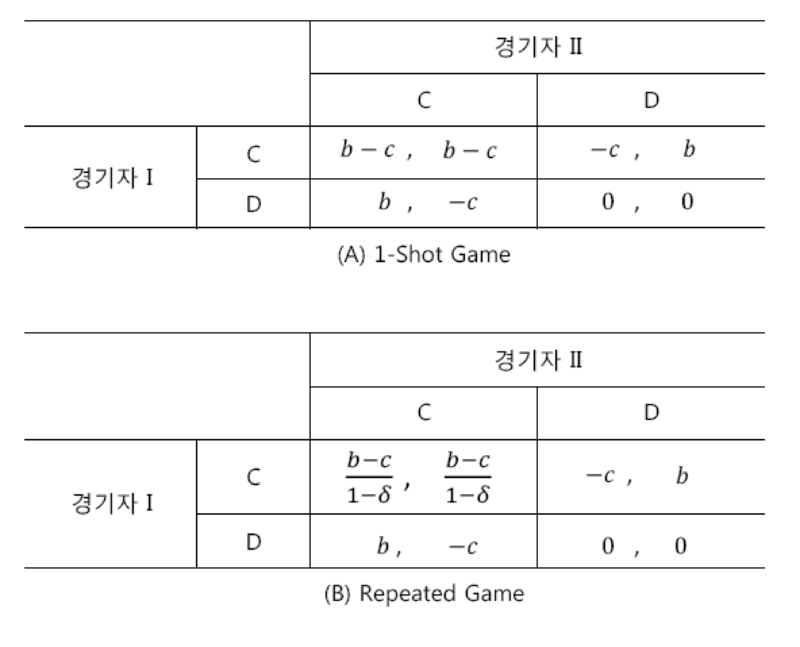
\includegraphics[width=2.5in]{repeat01.png}  
\end{center}
\end{frame}

\begin{frame}\frametitle{상호성 가설에 의한 이타적 행위 모형 V}%\vspace{5mm}
\begin{itemize}\large
\item 루소의 사슴사냥 게임 (stag hunt game): \\ 
\color{blue} $\rightarrow$ 조정게임 \\
\color{blue} $\rightarrow$ 죄수의 딜레마 게임이 반복되면 조정게임과 유사한 게임으로 변화 \\
%(2) 배신: 첫 회부터 배신을 하는 것으로 시작해서 계속 배신
\end{itemize}
\begin{center}
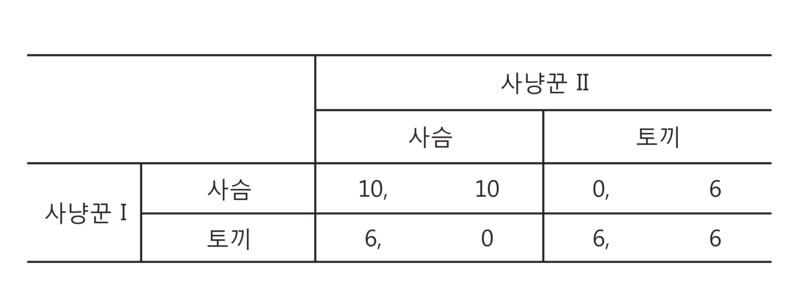
\includegraphics[width=3.5in]{staghunt01.png}
\end{center}
\end{frame}


\begin{frame}\frametitle{Axelrod's Computer Simulation I}\vspace{1em}
\begin{columns}[c]
\column{19em}
\begin{itemize}
\item 1980년, 정치학과 교수인 액설로드는 몇몇 게임이론가들에게 200회 동안 치러질 PDG의 전략의 설계를 부탁. 
\item 이들을 각각을 토너먼트에 붙이고 점수를 부여. 이 대결의 승자는? 
\item 생물학자인 Anatol Rapoport의 "TIT FOR TAT (TFT)" 
\item 이 결과가 발표되자 사람들은 놀랐다. 왜?
\\ 제출된 프로그램들 중에서 가장 단순한 4줄짜리 코드였기 때문. 
\end{itemize}
\column{11em}
\fbox{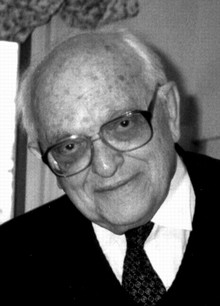
\includegraphics[width=11em]{Anatol_Rapoport.jpg}}
\end{columns}
\end{frame}

\begin{frame}\frametitle{Axelrod's Computer Simulation II}\vspace{2em}
\begin{columns}[c]
\column{17em}
\begin{itemize}
\item 이 사실이 학술지에 발표된 이후, 더 많고 다양한 전문가들에게 의뢰해 같은 모의 실험을 실시 
\item 두번째 라운드의 결과 역시 TFT가 가장 우수한 성적을 거두었다. 
\item 이후 RPDG 게임에서 협력을 가져온 좋은 해결책으로 TFT가 부상 
\end{itemize}
\column{13em}
\hspace{-1em}
\fbox{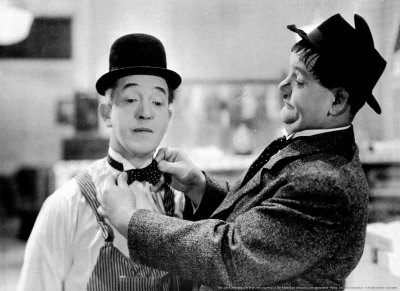
\includegraphics[width=13em]{tft.jpg}}
\end{columns}
\end{frame}

\begin{frame}\frametitle{Why TFT I}\vspace{1em}
\begin{columns}[c]
\column{17em}
\begin{enumerate}
\item Be nice:\\먼저 배신하지는 않는다. 
\item Be provocable: \\상대에게 호구가 되지 않는다. 
\item Don't be envious: \\상대보다 많은 보수를 바라지 않는다. 
\item Don't be too clever:\\충분히 예상 가능한 행보를 보여준다. 
\end{enumerate}
\column{13em}
\hspace{-1em}
\fbox{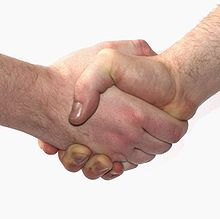
\includegraphics[width=13em]{hs.jpeg}}
\end{columns}
\end{frame}

\begin{frame}\frametitle{Why TFT II}\vspace{1em}
\begin{columns}[c]
\column{17em}
\begin{itemize}
\item 점수가 매겨진 방식을 생각해보자.  
\item 사실 TFT는 상대를 완전히 이긴 경우는 별로 없었다. 이겨도 그리 큰 차이로 이기지 않고, 져도 그리 크게 손해보지 않는 것. 
\item 만일 스포츠의 방식처럼 승자독식 방식이었다면?  
\item 아울러, 컴퓨터 알고리즘은 실수를 하지 않는다. 하지만 인간은 어떠한가? 
\end{itemize}
\column{13em}
\hspace{-1em}
\fbox{
\includegraphics[width=13em]{mistakes.png}}
\end{columns}
\end{frame}


\begin{frame}\frametitle{Trembling Hand I}
	\begin{itemize}\large
	\item 눈에는 눈, 이에는 이 TFT: \\ 
	\color{blue} 한 번의 실수는 상대방의 다음 전략에 영향을 미쳐 (C,D), (D,C) 쌍이 반복 \\ 
	%(2) 배신: 첫 회부터 배신을 하는 것으로 시작해서 계속 배신
	\end{itemize}
	\begin{center}
		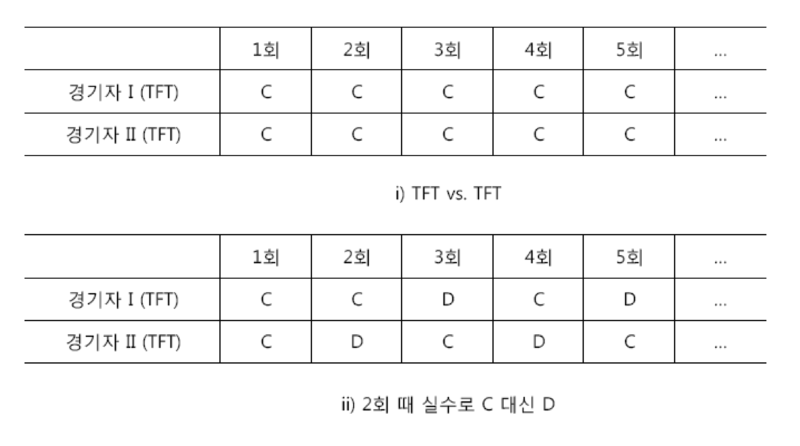
\includegraphics[width=4in]{tft01.png}
	\end{center}
\end{frame}

\begin{frame}\frametitle{Trembling Hand II}%\vspace{5mm}
\begin{itemize}\large
\item trigger 방아쇠 전략: \\ 
\color{blue} 한 번의 실수는 영원한 보복을 촉발하여 (D,D) 쌍이 반복 \\
%(2) 배신: 첫 회부터 배신을 하는 것으로 시작해서 계속 배신
\end{itemize}
\begin{center}
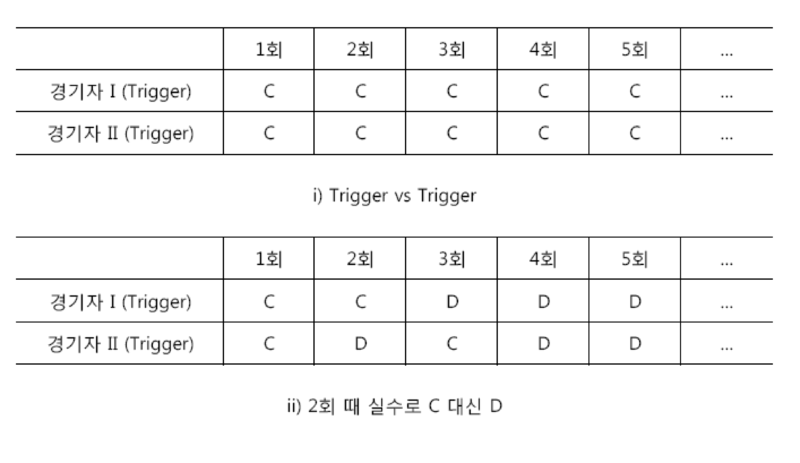
\includegraphics[width=4in]{trigger01.png}
\end{center}
\end{frame}

\begin{frame}\frametitle{Trembling Hand III}%\vspace{5mm}
\begin{itemize}\large
\item 'Win-Stay-Lose-Shift' (Pavlov 파브로프 전략): \\ 
(1) 내가 C 상대방도 C, 내가 만족 다음 기에도 C \\
(2) 내가 D 상대방은 C, 내가 만족 다음 기에도 D \\
(3) 내가 C 상대방은 D, 내가 불만족 전략을 바꿔서 D \\
(1) 내가 D 상대방은 D, 내가 불만족 전략 바꿔서 C \\
%(2) 배신: 첫 회부터 배신을 하는 것으로 시작해서 계속 배신
\end{itemize}
\begin{center}
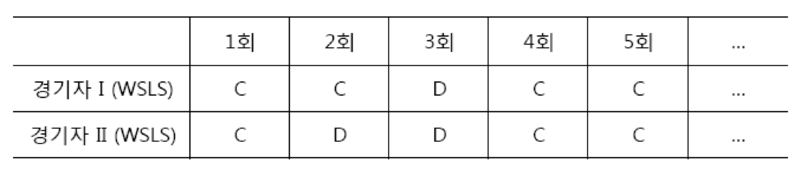
\includegraphics[width=4in]{pavlov01.png}
\end{center}
\end{frame}

\begin{frame}\frametitle{실제 사례 I}\vspace{2em}
\begin{columns}[c]
\column{16em}
\begin{itemize}
\item 현실에서 찾을 수 있는 가장 좋은 사례?
\item 삼성과 엘지, 진로와 하이트 
\item 이들은 경쟁관계이면서 협력관계 
\item 기업간 ``짬짜미''는 반복 게임의 좋은 사례 
\end{itemize}
\column{14em}
\fbox{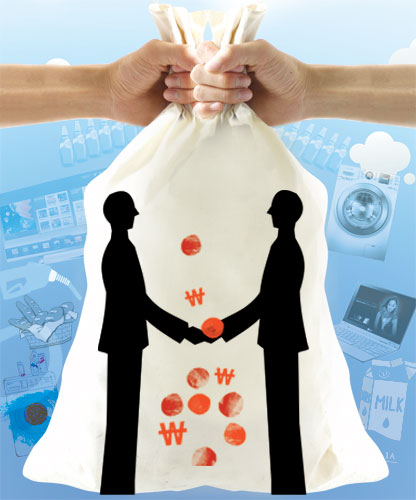
\includegraphics[width=12em]{collusion.jpg}}
\end{columns}
\end{frame}

\begin{frame}\frametitle{실제 사례 II}\vspace{2em}
\begin{columns}[c]
\column{16em}
\begin{itemize}
\item 덩어리가 너무 커서 배신에 따른 타격이 크다면?
\item 이 거래들을 여러 단계로 쪼개서, 전번 거래의 정보를 이번 거래에 활용한다. 
\item 왜 마약거래는 대부분 자잘하게 이뤄지는가? 
\end{itemize}
\column{14em}
\fbox{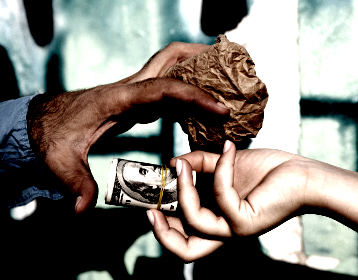
\includegraphics[width=12em]{drug.jpg}}
\end{columns}
\end{frame}

\begin{frame}\frametitle{실제 사례 III}\vspace{2em}
\begin{columns}[c]
\column{16em}
\begin{itemize}
\item 큰가시고기(stickleback fish)의 협력?
\item 포식자가 나타났을 때 이를 알아보기 위한 정찰이 필요
\item 포식자에 대한 접근을 반복 게임으로 나타낼 수 있다. 
\item Milinski는 이 점에 착안하여 큰가시고기의 협력 실험을 고안 
\end{itemize}
\column{14em}
\hspace{-1.5em}
\fbox{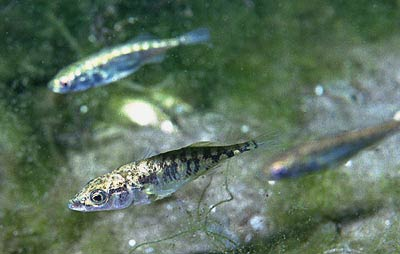
\includegraphics[width=14em]{stickle_2.jpg}}
\end{columns}
\end{frame}

\begin{frame}\frametitle{무한 반복게임은 언제나 좋은 결과를 낳을까?}\vspace{2em}
\begin{columns}[c]
\column{14em}
\begin{itemize}
\item IRG 자체가 좋은 결과를 낳는 것은 아니다. 
\item 사실 IRG는 어떤 균형이든 가능하게 한다. 
\item 옆의 예를 보자. 1-shot NE은 어디인가?
\item 만일 $\rho \geq  \frac{1}{2}$이고, GRIM을 쓰면 $(B,B)$도 균형으로 만들 수 있다!
\end{itemize}
\column{16em}
\begin{table}
\small
\setlength{\tabcolsep}{1.2em}
\begin{tabular}{|c|c|c|l|} \hline
& {A} &  {B} & {C} \\ \hline
{A} & {$2$}, {$2$} & {$2$}, {$1$} & {$0$}, {$0$}  \\ \hline%
{B} & {$1$}, {$2$} & {$1$}, {$1$} & {$-1$}, {$0$} \\ \hline%
{C} & {$0$}, {$0$} & {$0$}, {$-1$} & {$-1$}, {$-1$} \\
\hline
\end{tabular}
\end{table}
\end{columns}
\end{frame}

% section repeated_game (end)

\end{document}